\capitulo{4}{Discusión clínica.}
\section{Justificación clínica del problema.}

En esta sección se va exponer la fisiología de la mano humana y algunas patologías que afectan a su correcto funcionamiento.
\subsection{Fisiología de la mano.}

La mano es una estructura anatómica compleja, formada por cuatro sistemas, el sistema muscular, el sistema oseo, el sistema nervioso y el sistema articular. 

\subsubsection{Sistema muscular}

Esta formado por dos grupos principales de músculos, los extrínsecos y los intrínsecos, proporcionan la movilidad a la mano. 

Los músculos extrínsecos, son los músculos del antebrazo que se insertan en la mano. Los músculos intrínsecos son todos aquellos cuyos orígenes e inserciones están ubicadas en la región mano-muñeca, están subdivididos en cinco grupos tenares, hipotenares, lumbricales, interóseos palmares e interóseos dorsales . 

En la figura \ref{fig:Músculos_mano} , se pueden observar los músculos intrínsecos.
\begin{figure}
    \centering
    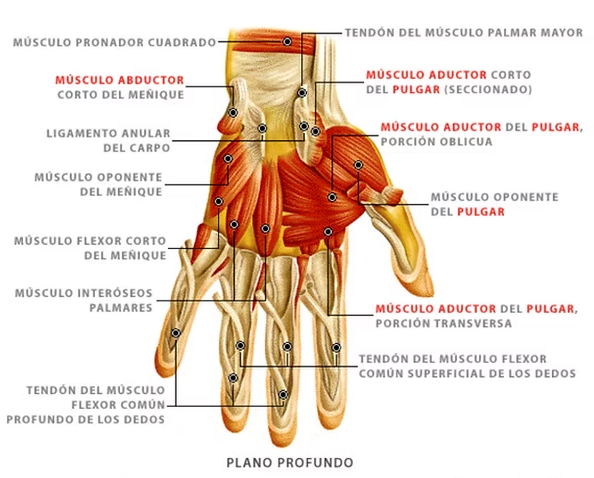
\includegraphics[width=0.5\linewidth]{img/Musculos_mano.png}
    \caption{Músculos intrínsecos de mano}
    \label{fig:Músculos_mano}
\end{figure}


\subsubsection{Sistema oseo}
La mano esta formada por 27 huesos, divididos en 3 grupos principales huesos del carpo, huesos del metacarpo y falanges de la mano.

Los huesos del carpo están dispuestos en dos filas distintas formando la muñeca, fila proximal (escafoides, semilunar, piramidal y pisiforme) y fila distal (trapecio, trapezoide, grande y ganchoso).

En la figura \ref{fig:Huesos_mano}, se pueden observar los 27 huesos que forman la mano.
\begin{figure}
    \centering
    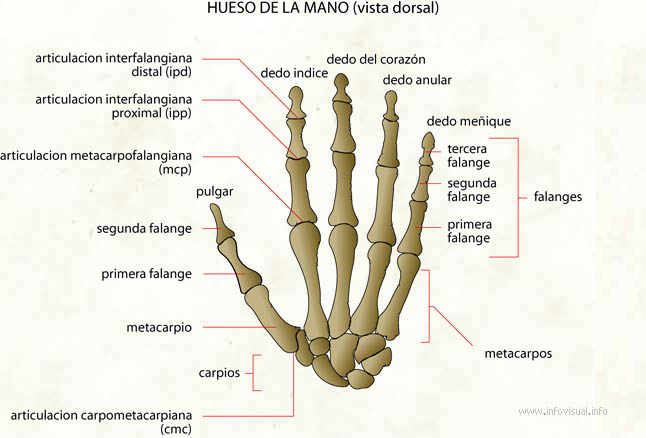
\includegraphics[width=0.6\linewidth]{img/Huesos_mano.png}
    \caption{Huesos de la mano. Fuente }
    \label{fig:Huesos_mano}
\end{figure}
\subsubsection{Sistema nervioso}

Los nervios de la mano y la muñeca se originan en el plexo braquial, son los nervios mediano, ulnar(bubital) y radial:
\begin{itemize}
    \item Mediano: atraviesa el túnel carpiano, responsable de la movilidad y sensibilidad de la palma y de los dedos anular, corazón , pulgar e indice.
    \item Ulnar: entra por los músculos flexores, responsable de la movilidad y sensibilidad de los músculos constrictivos de la mano y de los dedos meñique y anular.
    \item Radial: responsable de la sensibilidad de la mano.

En la figura \ref{fig:nervios de la mano}, podemos observar el recorrido y situación de los nervios desde el plexo braquial hasta la mano.
\begin{figure}
    \centering
    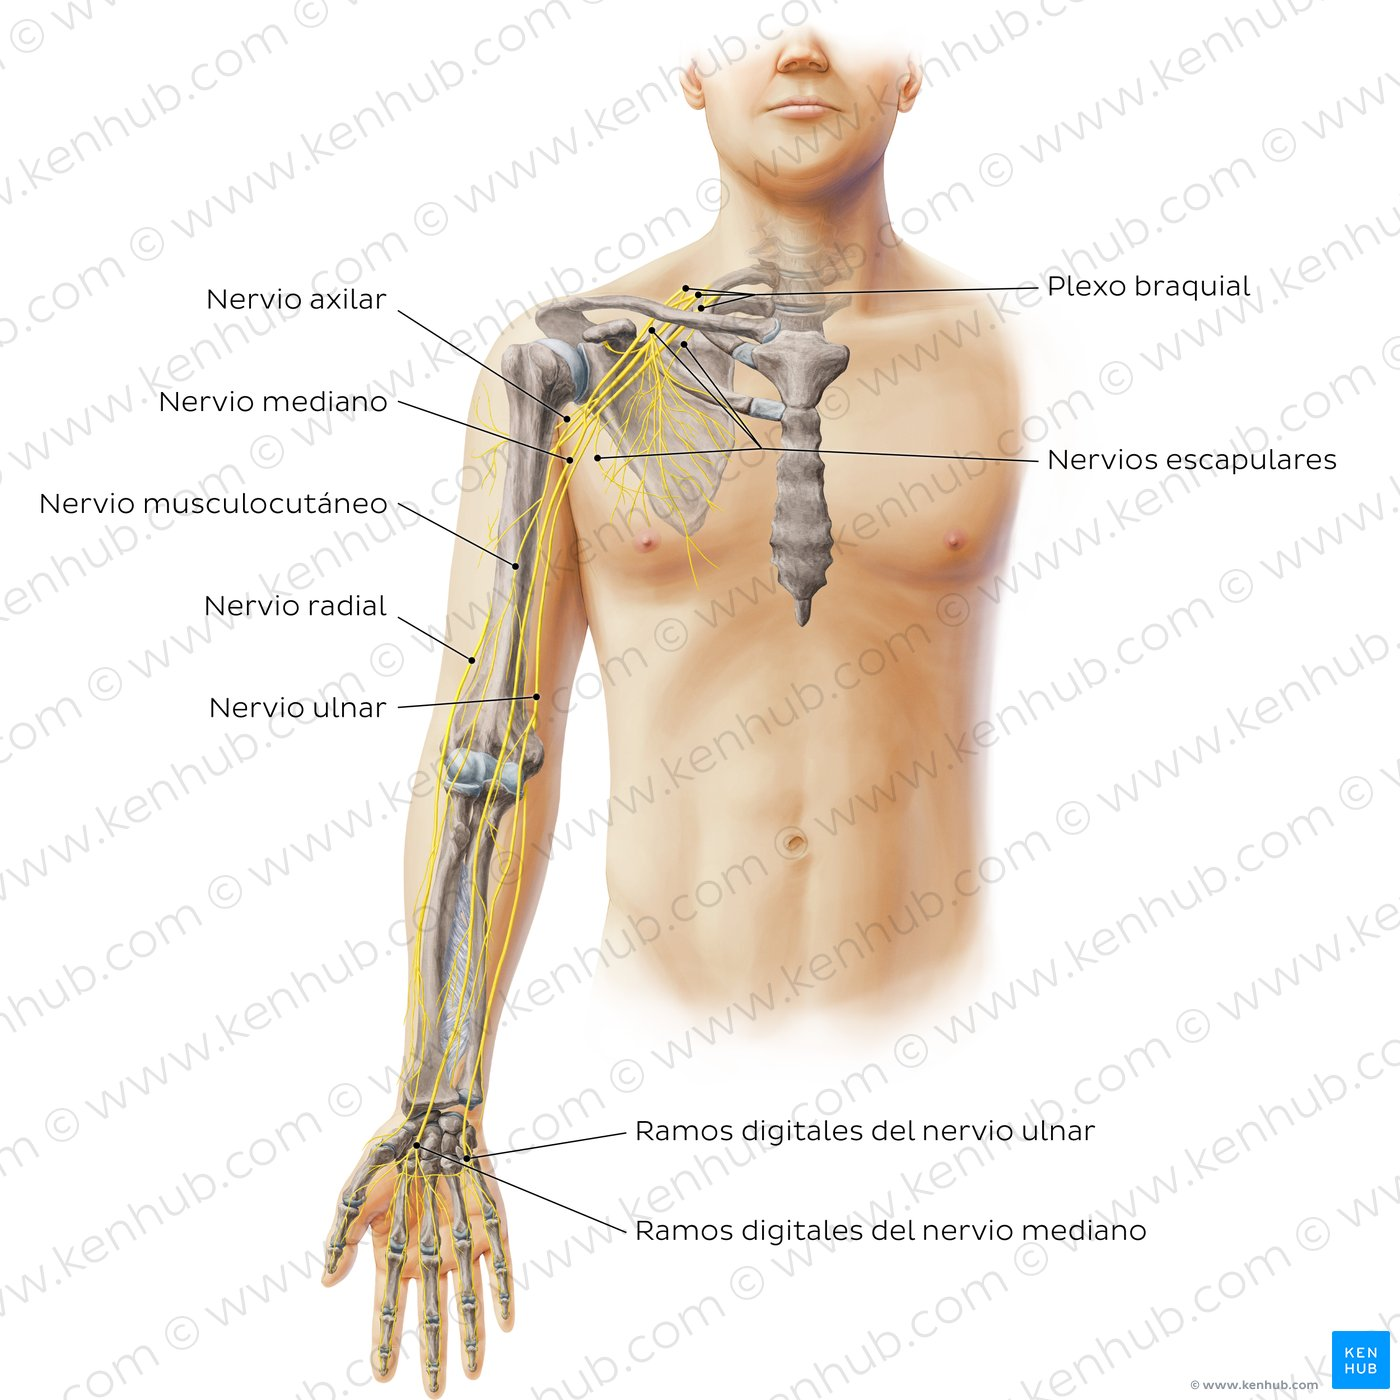
\includegraphics[width=0.5\linewidth]{img/Mano_nervios.png}
    \caption{Nervios de la mano. Fuente}
    \label{fig:nervios de la mano}
\end{figure}
\end{itemize}
\subsubsection{Sistema articular}

Son todas las articulaciones que comprenden desde la muñeca hasta las falanges. 

Las articulaciones entre el carpo y el metacarpo son las carpometacarpianas. Las articulaciones ente los metacarpos y las falanges proximales son las articulaciones metacarpofalángicas. Las articulaciones entre las falanges son las articulaciones interfalángicas - proximal y distal.
\subsection{Patologías que afectan a las manos.}

Entre el 6.6\% y el 28.6\% de las lesiones del sistema musculoesquelético son causadas en las manos.

En 2009 en Estados Unidos se trataron cerca de 100.000 lesiones en los miembros superiores, siendo los dedos y las muñecas las áreas mas afectadas, superando el 50\% de los casos.

Estas lesiones requieren de tratamientos especializados evitando complicaciones y discapacidades permanentes, recurriendo así a fisioterapeutas, terapeutas ocupacionales o médicos especializados en rehabilitación y fisioterapia.  
\subsubsection{Síndrome del túnel carpiano.}
Afectación en el nervio mediano de la muñeca, responsable de la sensibilidad y movimiento de partes de la mano.

Este síndrome es provocado por compresión del nervio  mediano dentro del túnel carpiano, produciendo entumecimiento, dolor, hormigueo, debilidad, o daño muscular en la mano y dedos. 

En la figura \ref{fig:Tunel_carpiano} se puede observar la localización del túnel carpiano y donde ocurre la compresión del nervio mediano que provoca la aparición de este síndrome. \cite{}
\begin{figure}
    \centering
    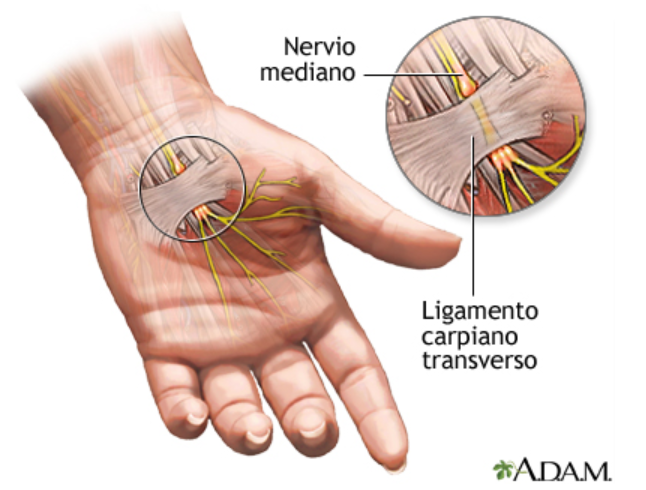
\includegraphics[width=0.5\linewidth]{img/Tunel_carpiano.png}
    \caption{Túnel carpiano. Fuente }
    \label{fig:Tunel_carpiano}
\end{figure}
\subsubsection{Síndrome de dolor regional complejo.}
Síndrome amplio que cubre los casos de inflamación y dolor crónico. Puede ocurrir en cualquier parte del cuerpo, pero generalmente afectan brazos, piernas, manos o pies. 

No está asociado a un daño de una estructura en específico, pero suelen ocurrir tras una lesión o evento médico, como una cirugía, un traumatismo, un accidente cerebrovascular o un ataque cardíaco. \cite{}

Los pacientes con este síndrome pueden experimentar algunos de estos síntomas: rigidez en las articulaciones afectadas, deterioro de la fuerza muscular y trastornos del movimiento, dolor repentino o no provocado que puede ser constante o cambiar con la actividad,dolor excesivo o duradero después del uso o contacto, adelgazamiento de un hueso o crecimiento óseo excesivo, sudoración y crecimiento de uñas y cabello de la articulación afectada, cambios en la textura de la piel o cambios en la temperatura y el color de la piel o hinchazón en la extremidad afectada.  \cite{}

\subsubsection{Rizartrosis.}
Es un tipo de artrosis que afecta únicamente al pulgar, es muy común a medida que se envejece. Se produce por el deterioro del cartílago de la articulación carpometacarpiana.

Entre los síntomas más comunes se encuentran el dolor intenso, inflamación y disminución de la fuerza y del rango de movimiento.

En la figura \ref{fig: Rizartrosis}, se puede observar el lugar de afectación de una forma más clara.

\begin{figure}
    \centering
    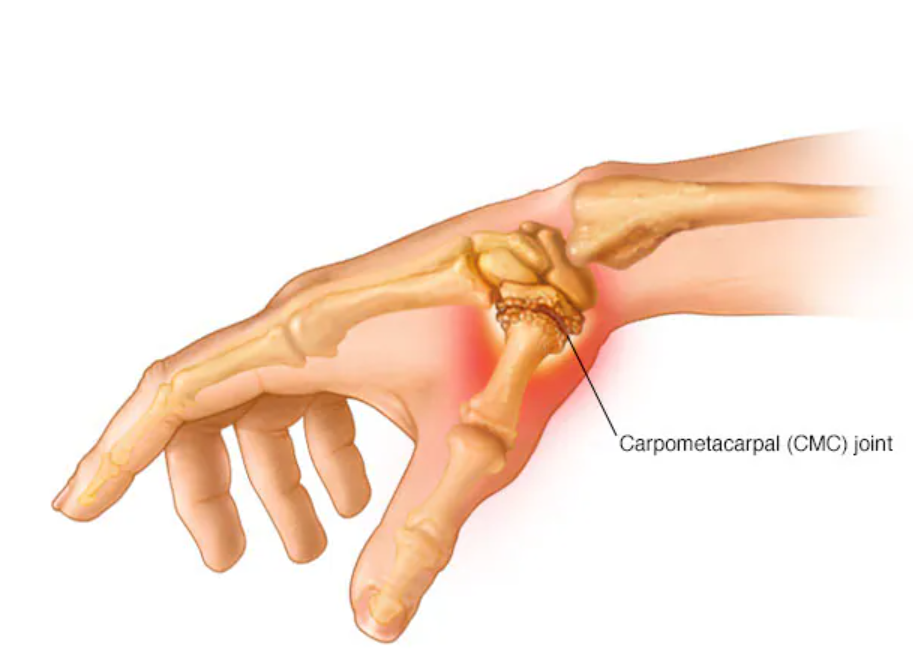
\includegraphics[width=0.5\linewidth]{img/Rizartrosis.png}
    \caption{Rizartrosis}
    \label{fig: Rizartrosis}
\end{figure}
\subsubsection{Tendinitis.}
Es la inflamación o descomposición de los tendones.

Suele afectar hombro, pie, muñeca, rodilla, tobillo o cuello, y se caracteriza por el dolor intenso (empeora con movimiento) o sensibilidad en la zona afectada. 

Las causas son muy amplias, pero suele ocurrir tras una lesión o sobrecarga.
\subsubsection{Fracturas.}

Son huesos rotos, causados por lesiones. Producen dolor, hinchazón, deformidades y/o deformidades.

Para su curación es necesario la inmovilización u operación de la rotura, lo que lleva a una pérdida de fuerza en el área afectada y en algunos casos en el desarrollo del síndrome de dolor regional complejo.
\subsubsection{Contractura de dupuytren.}
Contractura que se produce por la formación de nudos de tejido debajo de la piel de la mano, estos nudos acaban formando un cordón grueso que halan los dedos hacia la palma, quedando flexionados. 

No existen causas firmes, pero está demostrado que suele heredarse. 

Esta afectación es dolorosa e incapacita el uso de la mano, requiere de terapia y/o operaciones para revertir o frenar la flexión. 

En la figura \ref{fig:Dupuytrent}, se puede observar como avanza la contractura.

\begin{figure}
    \centering
    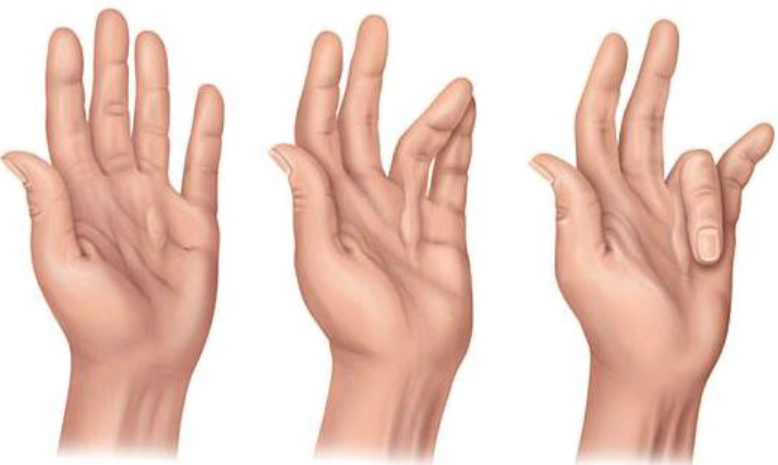
\includegraphics[width=0.5\linewidth]{img/Dupuytrent.png}
    \caption{Contractura de Dupuytrent. Fuente}
    \label{fig:Dupuytrent}
\end{figure}

\subsubsection{Enfermedades reumáticas.}
Las enfermedades reumáticas incluyen más de 200 enfermedades, tienen en común que se manifiestan en el aparato locomotor, o bien como un mecanismo basado en la respuesta inmune o inflamatoria excesiva. Ambas manifestaciones son acompañadas de dolor y discapacidad. 

\begin{itemize}
    \item Artrosis(osteoartritis): solo afecta a las articulaciones, generalmente en manos, rodillas,caderas, el cuello y la parte inferior de la espalda. Se rompe el cartílago y se vuelve áspero. Causa dolor, rigidez, inflamación y menor movimiento en las articulaciones. En las manos suele producir nódulos de Heberden o nódulos de Bouchard (figura \ref{fig:Nódulos}), que producen la malformación de las manos.

    \begin{figure}
        \centering
        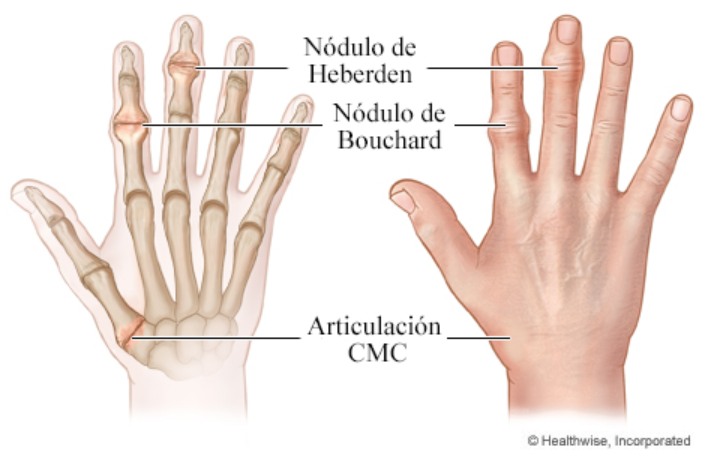
\includegraphics[width=0.75\linewidth]{img/Nodulos.png}
        \caption{Nódulos de Herbenden y Bouchard. Fuente}
        \label{fig:Nódulos}
    \end{figure}
    \item Artritis: Enfermedad autimune (sistema inmune ataca al tejido articular) que causa dolor, inflamación y rigidez en las articulaciones, en ocasiones se producen nódulos alrededor de ellas. 
    Muy común en muñeca y dedos
\end{itemize}

\subsubsection{Enfermedades neurológicas.}
Conjunto de enfermedades que afectan en una o más partes del sistema nervioso (cerebro, médula espinal o neuronas), existen más de 600. \cite{}

Sus causas son diversas e incluyen factores como genes defectuosos, problemas con el desarrollo del sistema nervioso, enfermedades degenerativas, enfermedades de los vasos sanguíneos, lesiones, trastornos convulsivos, cáncer o infecciones. \cite{}

La relación directa de los músculos con el sistema nervioso da como resultado que muchas de estas afectaciones se expresan en el movimiento, fuerza y/o agilidad del movimiento. 

Algunas que afectan a la movilidad, fuerza y/o agilidad de los miembros superiores: 
\begin{itemize}
    \item Accidente cerebrovascular
    \item Esclerosis múltiple
    \item Esclerosis lateral amiotrófica
    \item Lesiones en la médula
    \item Síndrome de Guillain-Barré
\end{itemize}

\section{Implicaciones terapéuticas.}
Las implicaciones terapéuticas son los efectos y consecuencias que implican un tratamiento o dispositivo sobre un paciente, pueden ser positivas o negativas.

El uso del dispositivo puede ser interdisciplinar, ya sea durante sesiones de terapia ocupacional o fisioterapia o, incluso durante las consultas médicas de revisión. 

El uso principal previsto es la monitorización continua de los pacientes. Este dispositivo puede utilizarse en diversos momentos de las sesiones, ya sea solo con los sensores o bien con la adaptación de mangos u otros soportes adaptados.

El proceso es bastante sencillo, el profesional sanitario debe registrar a los pacientes que desea monitorizar e ir registrando diariamente la fuerza que son capaces de realizar los pacientes. Esto permitirá a los profesionales observar si existe una evolución favorable, negativa o estancada y, en consecuencia,decidir si las sesiones deberían continuar o cesar. 

Otro uso relevante es la detección de la fatiga muscular durante las sesiones. Lo que permitiría realizar los cambios oportunos para la optimización total de las sesiones, o bien reducir el tiempo. La fatiga muscular se detectaría si al realizar mediciones en varias ocasiones durante las sesiones,se registran picos de fuerza significativamente más bajos en comparación con las anteriores.

\section{Contexto de uso real.}
El dispositivo está diseñado para un perfil de pacientes amplio, en edad, patología o afectación.

En cuanto al rango de edad, el dispositivo puede utilizarse desde adolescentes hasta personas mayores. Aunque no se ha probado en niños, no se recomienda su uso , debido a que los sensores tienen un diámetro de 3 cm, lo que dificulta al menor la correcta disposición de sus dedos, debido al tamaño de sus manos.

La integración del dispositivo durante una sesión de terapia ocupacional o fisioterapia es bastante amplia.

En el área de terapia ocupacional, la Tabla Canadiense se utiliza como parte de las sesiones de toda patología que implique una afectación en mano. En este punto de la sesión sería un buen momento para introducir el dispositivo, colocando los sensores en el mango e introducirlo en una de las varas de la tabla canadiense. 

A continuación, el profesional debe realizar los siguientes pasos: 
\begin{enumerate}
    \item Abrir la interfaz, iniciar sesión y seleccionar o registrar al paciente.
    \item Seleccionar empezar a medir y expresar al paciente que debe ejercer fuerza durante el tiempo que la luz led esté encendida.
    \item Visualización del nuevo registro y si se desea visualización de la gráfica. 
\end{enumerate}

En el área de fisioterapia, se podría realizar en cualquier parte de la sesión, ya sea solo o con algún soporte que se diseñe. Los pasos a realizar serían iguales que en los de una sesión de terapia ocupacional. 
\begin{enumerate}
    \item Abrir la interfaz, iniciar sesión y seleccionar o registrar al paciente.
    \item Seleccionar empezar a medir y expresar al paciente que debe ejercer fuerza durante el tiempo que la luz led esté encendida.
    \item Visualización del nuevo registro y si se desea visualización de la gráfica. 
\end{enumerate}

Además, se podría utilizar durante las revisiones médicas, durante el reconocimiento. Pudiendo el médico visualizar si de una revisión a otra existen cambios. 

\section{ Comparativa con estudios o protocolos clínicos existentes.}

A partir de los estudios revisados en la sección 'Estado del arte' del apartado 'Conceptos teóricos', se va a comparar los estudios, prototipos o protocolos existentes con la propuesta presentada con este proyecto, destacando ventajas, limitaciones y diferencias.

En los diseños analizados (Juliana Gomez et al, Luis Carlos Ralon Gordillo y el mio proprio) , existe un objetivo común de la monitorización de la fuerza ejercida por pacientes en terapia de mano. 

Aunque en los 3 se utiliza el sensor de fuerza resistivos(FSR) como elemento principal, podemos observar diferencias claras entre los estudios. En la tabla \ref{tab:comparativa_prototipos} se presenta una tabla comparativa de los 3 dispositivos.
\begin{table}[h]
    \begin{tabular}{|p{2cm}|p{4cm}|p{4cm}|p{4cm}|}
    \hline
    \rowcolor[HTML]{BFBFBF} 
    \textbf{Aspecto} & \textbf{Juliana Gómez et al.} & \textbf{Luis Carlos Ralón Gordill}& \textbf{Diseño propio} \\ \hline
    Sensor utilizado & FSR & FSR & FSR \\ \hline
    Número de sensores & 5 & 1 & 5 \\ \hline
    Uso del resorte & Transmisión de fuerza & Generar resistencia & No aplica \\ \hline
    Mecanismo de transmisión & Mediante resorte & Mediante resorte& Directo \\ \hline
    Ventajas & Alta precisión & Uso en niños & Uso aplicabilidad múltiple\\ \hline
    Limitaciones & Solo permite el agarre de precisión & Fallos en Resorte-Sensor & . \\ \hline
    Coste  & No menciona & No menciona precio exacto, pero deja claro que busca producir el menos coste y al utilizar un único sensor el coste total es bajo. & Menor posible,  \\ \hline
    \end{tabular}
    \caption{Comparativa de prototipos}
    \label{tab:comparativa_prototipos}
\end{table}

\section{Limitaciones y riesgos clínicos.}
Este dispositivo presenta un perfil de seguridad óptimo para su uso clínico, no supone ningún riesgo para pacientes o profesionales sanitarios. 

Los sensores que incorpora, son sensores resistentes al agua, que permite una desinfección rápida, óptima y efectiva entre pacientes mediante el uso de toallitas o paños húmedos con desinfectante. Siempre evitando que se sumerjan completamente en cualquier solución líquida, debido a que son componentes eléctricos.

Si se añaden accesorios:
\begin{itemize}
    \item Mango impresión 3D: su desinfección depende mucho del material con el que se ha impreso. Si utilizamos PLA (material pensado debido a su bajo coste), no debemos utilizar desinfectantes que contengan acetonas ya que este producto es capaz de degradarlo. Se podrían usar toallitas antibacterianas o paños humedecidos en soluciones desinfectantes.
    \item Otros soportes: se deben desinfectar según las especificaciones del material del que estén fabricados para no degradarlo.  
\end{itemize}

Un protocolo de limpieza adecuado garantiza las condiciones higiénicas necesarias para un uso seguro y continuado sin comprometer la salud de los pacientes o de los sanitarios que lo manipulen.